%Corps du document :
%\setlength{\parindent}{1cm}    

\section{Répartition des composants sur l'architecture n-tiers}

\subsection{Répartition des blocs applicatifs}

Les blocs \textbf{Produits}, \textbf{Client} et \textbf{Agence} seront implémentés sur le serveur du site central, mais également répliqués sur les serveurs des agences principales. L'architecture de ces données sera en \textbf{multi-maître}. Ainsi, chaque site pourra modifier les données. La gestion des conflits se fera si possible automatiquement, puis au besoin par l'intervention d'un responsable sur le site central.

Les blocs \textbf{Agence} et \textbf{Client}, en plus d'être répliqués, seront répartis. La base de données de chaque agence contiendra seulement les informations des sous-agences qu'elle gère.

Même si les modifications de \textbf{Client} sont nombreuses, peu de conflits seront générés car peu de modifications seront émises à partir du site central. L'intérêt de cette réplication est la sauvegarde des données du client, et un accès aux données accéléré.

Les blocs \textbf{Agenda} et \textbf{Contact} seront répartis. Aucune information ne sera sur le site central. Chaque agence principale gèrera ces propres informations.

\begin {center}
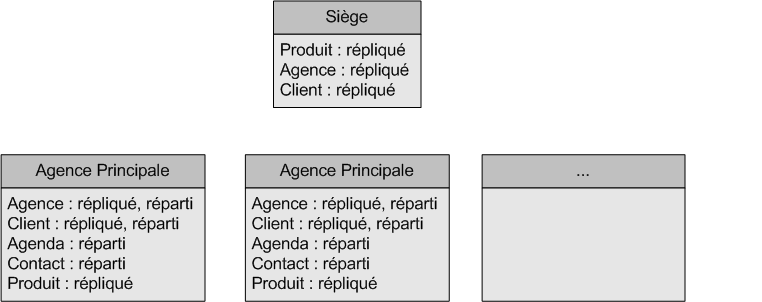
\includegraphics[width=\textwidth]{repartition_bloc.png}
\end {center}

\subsection{Principaux flux applicatifs échangés}

\subsubsection{Consultation des données}

Lorsqu'une donnée est requise par l'une des agences, elle tente si possible de la récupérer sur ses
propres serveurs, ou émet une requète à l'agence principale à laquelle elle est affectée. Celle-ci
peut soit posséder cette donnée, soit la demander au site central, et la mettre en cache. Les systèmes
de cache sont très régulièrement rafraichis afin d'éviter de travailler sur des données trop anciennes
de minimiser le plus possible le risque de conflits (voir les mécanismes de réplication ci-après).

\subsubsection{Mise à jour des données}

\paragraph{Mise à jour active}

Lorsqu'une donnée est mise à jour sur les serveurs d'une agence, et que ces derniers connaissaient les
agences sur lesquelles la donnée est répliquée, ils émettent directement une notification pour les
prévenir du changement.

\paragraph{Mise à jour passive}

Lorsqu'un serveur ne sait pas où se trouvent toutes les copies de ses données, un mécanisme de mise à
jour passive des données intervient. Toutes les données répliquées sont brassées régulièrement,
et transférées de manière routinière entre les agences pour que le système maintienne sa cohérence au
mieux possible tout en veillant à ne pas surcharger le réseau inter-agences.

\subsubsection{Réplication des données}

Pour une plus grande rapidité d'accès, les données considérées comme globales sont répliquées entre les
agences. Elles sont mises à jour le plus régulièrement possible pour garantir la fraîcheur des données
et limiter les risques de conflits.

\paragraph{Réplication descendante}

Comme indiqué précédemment, les données des blocs \textbf{Produits}, \textbf{Client} et \textbf{Agence}
sont répliquées depuis le site central vers les serveurs des agences principales.

\paragraph{Réplication montante}

Il existe également un mécanisme de réplication des données des agences principales vers le site central,
afin que celui-ci puisse conserver des sauvegardes globales (voir paragraphe suivant). De la même façon,
les sous-agences répliquent leurs données vers les agences principales auxquelles elles sont affectées.
Cette réplication montante ne concerne pas les blocs applicatifs \textbf{Agenda} et \textbf{Contact}, car
ils relèvent de la responsabilité des sous-agences seules.

\subsubsection{Sauvegarde des données}

Les données sont systématiquement et régulièrement sauvegardées.

\paragraph{Restauration intégrale à froid}

Celles qui sont présentes ou répliquées
sur le site central sont enregistrées sous forme de clichés instantanés, qui peuvent être restaurés
intégralement à froid en cas de problème majeur (cas extrêmes comme la perte d'un ou plusieur serveurs).

\paragraph{Restauration partielle localisée à chaud}

Un mécanisme de restauration partielle à chaud est également prévu pour
les problèmes de pertes de données localisées, comme la perte d'un dossier ou la corruption d'une entrée
au sein d'une base de données. Ce mécanisme est géré automatiquement par notre système de Base de Données.

Il existe des systèmes de sauvegardes similaires au sein de chaque agence.
